\documentclass[11pt,twocolumn]{article}
\usepackage[margin=0.72in]{geometry}
\usepackage{amsmath,amssymb,amsthm}
\usepackage{booktabs}
\usepackage{graphicx}
\usepackage{hyperref}
\usepackage{xcolor}
\usepackage{enumitem}

\hypersetup{
  colorlinks=true,
  linkcolor=blue!60!black,
  citecolor=green!45!black,
  urlcolor=blue!65!black
}

\newtheorem{proposition}{Proposition}
\newtheorem{definition}{Definition}

\newcommand{\ZZ}{\mathbb{Z}}
\newcommand{\NN}{\mathbb{N}}

\title{\textbf{Machine-Checked Exact-Integer Certificates for Normal and Mis\`ere Grid NoGo, Coins-are-Lava, and Subcubic Bipartite Graph NoGo PSPACE-Completeness}}
\author{Lluis Eriksson\thanks{Independent researcher; manuscript prepared with transparent AI assistance via Google Antigravity. Source code, Lean~4 proofs, and exact certificates: \url{https://github.com/lluiseriksson/nogo-pspace-certificates}.}}
\date{November 25, 2026}

\begin{document}
\maketitle

\begin{abstract}
Kyle Burke, Alfie Davies, and Craig Tennenhouse (\texttt{arXiv:2611.33127}, November 24, 2026) resolved the open problem of Burke and Hearn (2019), proving that \textsc{NoGo} is PSPACE-complete on positions reachable from an empty $n \times n$ square grid under both normal play and mis\`ere play (Theorem~1.1) via direct square-grid Bounded Two-Player Constraint Logic (B2CL) reductions, and proving that \textsc{Graph NoGo} remains PSPACE-complete under normal play on connected bipartite subcubic ($\Delta \le 3$) graphs (Theorem~1.2) via a new \textsc{Coins-are-Lava} edge-removal game (Lemma~4.1). We present a machine-checked, zero-floating-point formalization and exact combinatorial game-tree auditor for the finite budget, truth-table, reachability, rope-majority, and parity-win core of these results. First, an 18-theorem zero-dependency Lean~4 kernel (\texttt{NoGoPSPACE.lean}, Lean~4.35.0; 0~\texttt{sorry}, 0~warnings, 0~\texttt{Classical.choice}, 9 zero-axiom theorems) formalizes the B2CL move budget $x = a + 2b + c + d + 3e$, White reserve hole capacity, empty-board alternating parity, game-tree depth bounds, normal-vs.-mis\`ere terminal and wire-signal duality, exact AND/OR/SPLIT/CHOICE truth tables, Lemma~4.1 clause/formula majorities, odd-parity cut shifts, rope-width separation $2tw+1 < (2t+3)w$, and subcubic bipartiteness. Second, \texttt{NOGO-PSPACE-CERT-1.0} audits four exact modes—empty-board reachability replay, normal/mis\`ere grid minimax, \textsc{Coins-are-Lava} minimax, and connected bipartite subcubic Graph NoGo—replaying 16 canonical certificates in $0.060$--$6.495\,\mathrm{ms}$ and rejecting 60/60 live adversarial forgeries.
\end{abstract}

\section{Introduction}
\textsc{NoGo} is the two-player combinatorial placement game derived from \textsc{Go} by forbidding both captures (including self-captures) and passes~\cite{burke2019pspace,hearn2009games}. Following the PSPACE-completeness of planar \textsc{Graph NoGo}~\cite{burke2019pspace} and \textsc{Dots \& Boxes}~\cite{buchin2021dots}, Burke, Davies, and Tennenhouse~\cite{burke2026nogo} settled two major open questions:
\begin{enumerate}[leftmargin=*,nosep]
  \item \emph{Square-grid normal \& mis\`ere play (Theorem~1.1):} Realizing B2CL gadgets (\textsc{Goal}, \textsc{Variable}, \textsc{Or}, \textsc{And}/\textsc{Split}, \textsc{Choice}) directly on $n \times n$ grids with insulated White wires, frozen liberties, and a checkerboard White reserve yields PSPACE-completeness on positions reachable from the empty grid under both normal and mis\`ere play.
  \item \emph{Subcubic bipartite graphs (Theorem~1.2 \& Lemma~4.1):} Introducing \textsc{Coins-are-Lava} (a Strings-and-Coins~\cite{demaine2021strings} variant forbidding isolating any coin), proving its PSPACE-completeness from Schaefer's positive-CNF game via odd rope widths $N = 2t+3$, and reducing to connected bipartite graphs of maximum degree $\Delta \le 3$.
\end{enumerate}

\paragraph{Contributions and Scope.}
We formally verify and audit the finite combinatorial, algebraic, truth-table, parity, and exact minimax core of~\cite{burke2026nogo}. We explicitly scope our Lean~4 kernel away from full Turing-machine PSPACE reductions, planar grid layout routing, and asymptotic polynomial-size circuit constructions:
\begin{enumerate}[leftmargin=*,nosep]
  \item \textbf{Zero-dependency Lean~4 kernel (\S\ref{sec:lean}):} 18 constructive theorems in \texttt{NoGoPSPACE.lean} (Lean~4.35.0~\cite{demoura2021lean4}), 0~\texttt{sorry}, 0~warnings, 0~\texttt{Classical.choice}, and \textbf{9 zero-axiom theorems}.
  \item \textbf{Pure-stdlib exact game verifier (\S\ref{sec:certifier}):} \texttt{NOGO-PSPACE-CERT-1.0}, auditing grid reachability, normal/mis\`ere minimax, \textsc{Coins-are-Lava}, and subcubic bipartite Graph NoGo with zero floats.
  \item \textbf{Empirical atlas \& red-team audit (\S\ref{sec:results}):} 16 canonical certificates ($0.060$--$6.495\,\mathrm{ms}$), exact normal-vs.-mis\`ere winner flips on grids ($2\times 2, 2\times 4$) and subcubic bipartite graphs ($K_{3,3}, Q_3, L_8$), rope-separation scaling, and 60/60 rejected live adversarial forgeries.
\end{enumerate}

\section{Budget, Rope-Width, and Parity Invariants}\label{sec:prelim}
In Section~2 of~\cite{burke2026nogo}, a B2CL circuit with $a$ \textsc{Variable}, $b$ \textsc{Or}, $c$ \textsc{And}, $d$ \textsc{Split}, and $e$ \textsc{Choice} gadgets prescribes
\begin{equation}
  x = a + 2b + c + d + 3e
  \label{eq:budget}
\end{equation}
Black moves; a checkerboard White reserve with $x+1-a$ non-adjacent holes yields $x-a$ waiting moves alongside White's $a$ \textsc{Variable} plays, so Black wins going first iff Black claims the extra \textsc{Goal} move ($x+1 > x$). In Section~4 (Lemma~4.1), a positive-CNF formula with $c$ clauses and $n$ variables is encoded into $2c-1$ rows (each $k$-literal clause padded by $k-1$ copies of $1$ to $2k-1$ entries) joined by ropes of widths $1, N, N^2, N^3, N^4$ with odd $N = 2t+3$. At every width~$w$, at most $2tw+1$ lower-level cuts occur before completion, strictly below $Nw$:
\begin{equation}
  2tw + 1 < (2t+3)w = Nw,
  \label{eq:rope}
\end{equation}
and from an odd initial string total $M = 2k+1$, a False chosen entry leaves an odd count $R_{\mathrm{F}} = 2(c+n+1)+1$ (even cuts, White wins), whereas a True entry allows one extra cut to ground~$g$, leaving $R_{\mathrm{T}} = 2(c+n+1)$ (odd cuts, Black wins).

\section{Zero-Dependency Lean 4 Kernel}\label{sec:lean}
We formalize 18 constructive theorems in \texttt{lean/NoGoPSPACE.lean} (Lean~4.35.0, zero external dependencies), audited via \texttt{lean/AuditAxioms.lean} with 0~warnings, 0~\texttt{sorry}, 0~\texttt{Classical.choice}, and 0~\texttt{Lean.ofReduceBool} (Table~\ref{tab:lean}).

\begin{proposition}[Constructive NoGo PSPACE Kernel]\label{prop:lean}
\leavevmode
\begin{enumerate}[leftmargin=*,nosep]
  \item \emph{Normal-play budget \& reachability (Theorems~1--4):} Exact B2CL move balance $a+(x-a)=x < x+1$, White reserve capacity, even empty-board alternating parity $(|B|+|W|)\equiv 0 \pmod 2$, and game-tree depth $\le |V|-s_0$.
  \item \emph{Normal/mis\`ere duality \& B2CL gates (Theorems~5--11):} Terminal outcome duality, wire-signal inversion, exact \textsc{And}, \textsc{Or}, \textsc{Split}, and \textsc{Choice} truth tables, and mis\`ere \textsc{Or}/\textsc{And} move-saving implication.
  \item \emph{\textsc{Coins-are-Lava} \& subcubic graphs (Theorems~12--18):} Clause and formula strict majorities, odd-to-even parity flip~\eqref{eq:rope}, rope-width separation $2tw+1 < (2t+3)w$, subcubic bipartite degree/coloring invariant, legal cut invariant $\deg(u),\deg(v) \ge 2$, and concrete Figure~6 / Section~4 sanity checks.
\end{enumerate}
\end{proposition}

\begin{table}[t]
\centering
\caption{Complete 18-theorem Lean~4.35.0 kernel in \texttt{NoGoPSPACE.lean} (0~\texttt{sorry}, 0~warnings, 0~\texttt{Classical.choice}, 9 zero-axiom theorems).}
\label{tab:lean}
\resizebox{\columnwidth}{!}{%
\begin{tabular}{@{}rll@{}}
\toprule
\# & Lean~4 Theorem Identifier & Axiom Footprint \\
\midrule
1 & \texttt{normal\_play\_move\_budget\_exact} & \texttt{[propext]} \\
2 & \texttt{white\_reserve\_hole\_capacity} & \texttt{[propext, Quot.sound]} \\
3 & \texttt{empty\_board\_reachability\_parity} & \texttt{[propext]} \\
4 & \texttt{nogo\_game\_tree\_depth\_bound} & \texttt{[propext, Quot.sound]} \\
5 & \texttt{normal\_vs\_misere\_terminal\_duality} & \texttt{none} \\
6 & \texttt{normal\_vs\_misere\_wire\_inversion} & \texttt{none} \\
7 & \texttt{b2cl\_and\_gate\_truth\_table} & \texttt{none} \\
8 & \texttt{b2cl\_or\_gate\_truth\_table} & \texttt{none} \\
9 & \texttt{b2cl\_split\_gate\_duality} & \texttt{none} \\
10 & \texttt{b2cl\_choice\_gate\_exclusivity} & \texttt{none} \\
11 & \texttt{misere\_or\_and\_gate\_exact} & \texttt{none} \\
12 & \texttt{coins\_are\_lava\_clause\_majority} & \texttt{[propext]} \\
13 & \texttt{coins\_are\_lava\_formula\_majority} & \texttt{none} \\
14 & \texttt{coins\_are\_lava\_odd\_parity\_shift} & \texttt{[propext]} \\
15 & \texttt{coins\_are\_lava\_rope\_majority\_win} & \texttt{[propext]} \\
16 & \texttt{subcubic\_bipartite\_degree\_bound} & \texttt{[propext, Quot.sound]} \\
17 & \texttt{legal\_cut\_degree\_invariant} & \texttt{[propext, Quot.sound]} \\
18 & \texttt{nogo\_gadget\_budget\_concrete\_check} & \texttt{none} \\
\bottomrule
\end{tabular}}
\end{table}

\section{Exact Game-Tree Verifier}\label{sec:certifier}
\texttt{NOGO-PSPACE-CERT-1.0} (\texttt{src/nogo\_certifier.py}) is a pure-stdlib zero-float verifier enforcing strict JSON types and exact BFS group-liberty rules across four modes:
\begin{enumerate}[leftmargin=*,nosep]
  \item \textbf{Mode~1 (\texttt{nogo\_board\_legality\_\allowbreak and\_reachability}):} Replays an even-length alternating sequence from an empty $r \times c$ grid, verifying no capture/suicide at every ply and exact Black/White legal move counts.
  \item \textbf{Mode~2 (\texttt{b2cl\_gadget\_minimax\_\allowbreak normal\_misere}):} Solves exact normal or mis\`ere minimax on grid NoGo positions ($\le 12$ empty cells) and verifies the winning first move preserves the winning strategy.
  \item \textbf{Mode~3 (\texttt{coins\_are\_lava\_\allowbreak exact\_minimax}):} Solves exact \textsc{Coins-are-Lava} minimax on multigraphs (up to 16 coins, 18 strings), enforcing $\deg(u),\deg(v)\ge 2$ on every cut and verifying the winning first cut.
  \item \textbf{Mode~4 (\texttt{subcubic\_bipartite\_\allowbreak graph\_nogo}):} Verifies graph simplicity, connectivity, 2-colorability, and $\Delta \le 3$, then solves exact normal-play \textsc{Graph NoGo} minimax and verifies the winning move.
\end{enumerate}

\section{Empirical Atlas and Red-Team Audit}\label{sec:results}
Running \texttt{scripts/run\_all\_experiments.py} generates 16 canonical certificates (4 per mode) and four exact game-tree sweeps, verified end-to-end by \texttt{scripts/verify\_all.py} with SHA-256 manifest checks across all 41 tracked artifacts.

\begin{figure}[t]
  \centering
  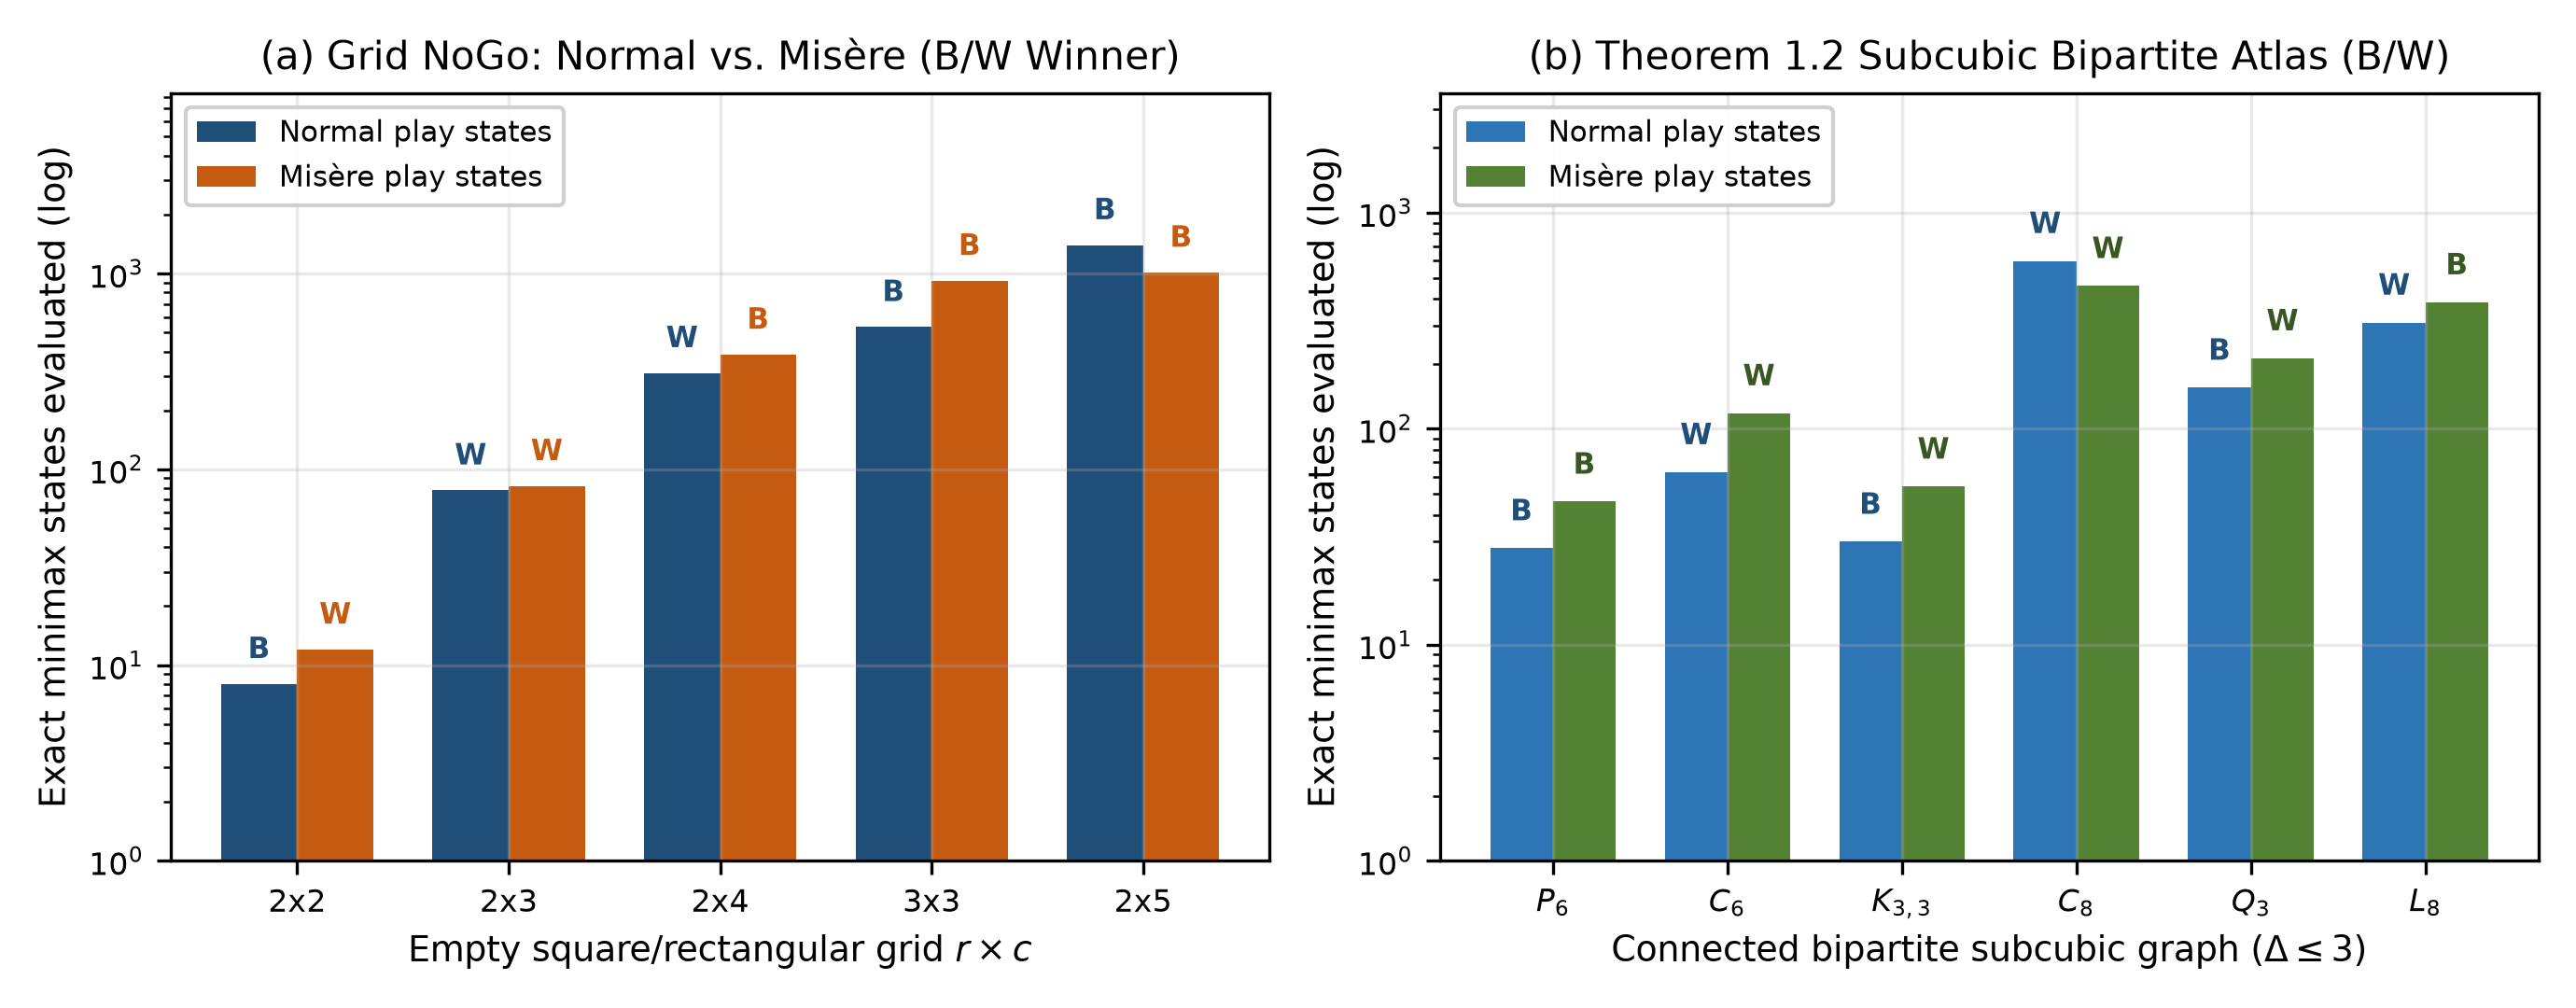
\includegraphics[width=\columnwidth]{../figures/fig1_grid_normal_vs_misere_and_subcubic.png}
  \caption{(a) Exact normal vs.\ mis\`ere minimax state counts and B/W winners across empty grids ($2\times 2$ through $2\times 5$), showing winner flips on $2\times 2$ and $2\times 4$. (b) Theorem~1.2 connected bipartite subcubic ($\Delta \le 3$) Graph NoGo atlas, showing winner flips on $K_{3,3}$, $Q_3$, and $L_8$.}
  \label{fig:minimax}
\end{figure}

\paragraph{Grid Minimax and Subcubic Bipartite Atlas (Fig.~\ref{fig:minimax}).}
On empty square/rectangular grids, exact minimax reveals sharp normal-vs.-mis\`ere reversals: on $2\times 2$, Black wins normal play ($8$ states) while White wins mis\`ere ($12$ states); on $2\times 4$, White wins normal ($310$ states) while Black wins mis\`ere ($385$ states); on $3\times 3$, Black wins both ($533$ states, $4.979\,\mathrm{ms}$ normal; $918$ states, $6.495\,\mathrm{ms}$ mis\`ere) but the winning opening move shifts from corner vertex~$0$ to center vertex~$4$. Across six connected bipartite subcubic graphs ($P_6, C_6, K_{3,3}, C_8, Q_3, L_8$), exact normal-vs.-mis\`ere winners flip on 3/6 graphs, including non-planar $K_{3,3}$ (Black normal, $30$ states vs.\ White mis\`ere, $54$ states) and 3-cube $Q_3$ (Black normal, $155$ states vs.\ White mis\`ere, $212$ states).

\begin{figure}[t]
  \centering
  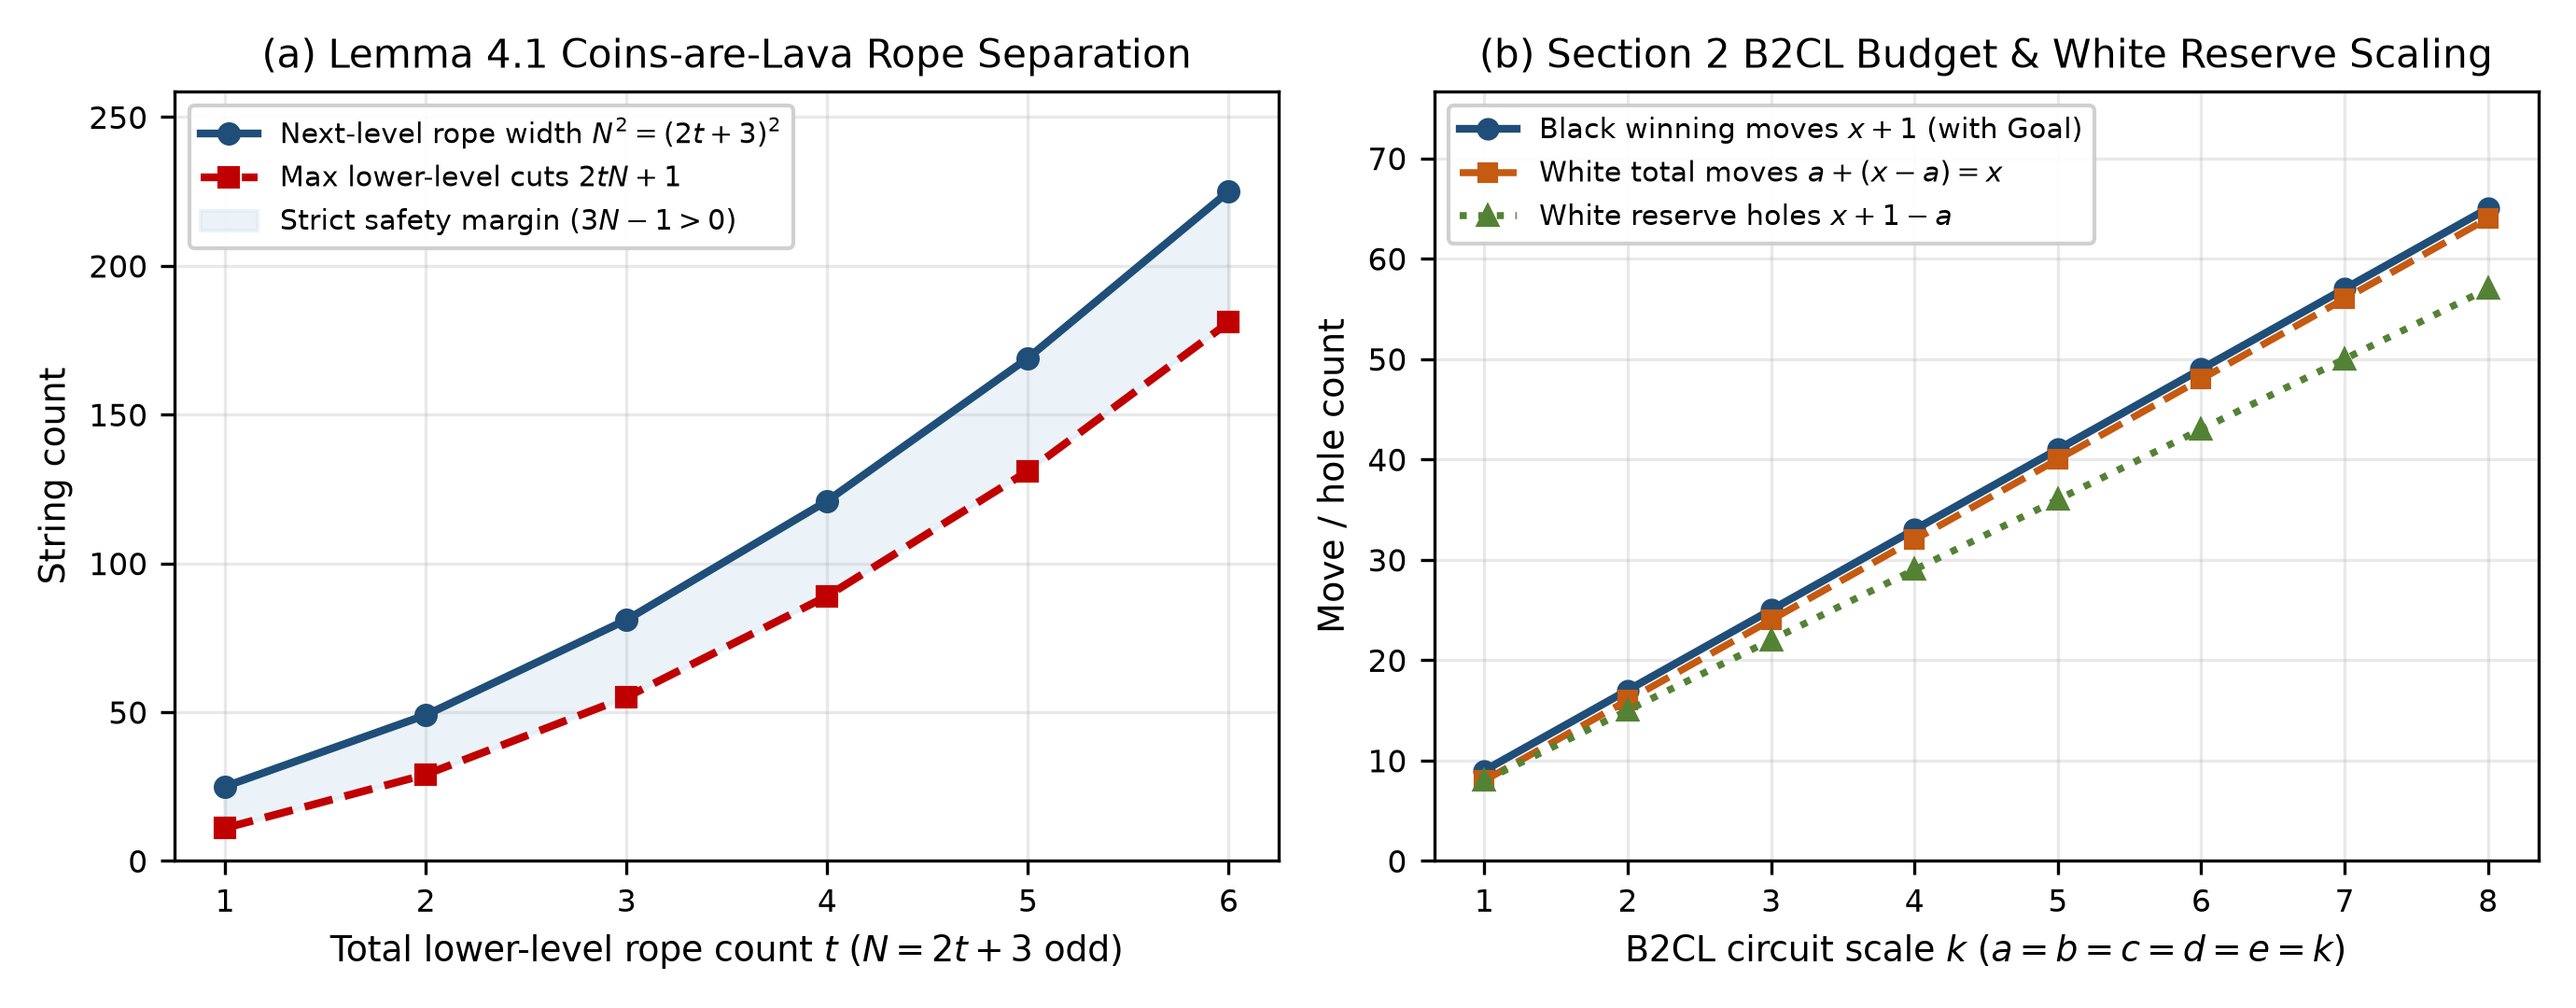
\includegraphics[width=\columnwidth]{../figures/fig2_lava_rope_and_b2cl_budget.png}
  \caption{(a) Exact Lemma~4.1 rope-width separation $2tN + 1 < N^2$ for $N = 2t+3$ ($t=1\dots 6$), guaranteeing safety margin $3N-1 > 0$. (b) Exact Section~2 B2CL move budget $x = a+2b+c+d+3e$, White reserve holes $x+1-a$, and Black's $+1$ Goal margin.}
  \label{fig:rope}
\end{figure}

\paragraph{Reachability, \textsc{Coins-are-Lava}, and B2CL Budgets (Fig.~\ref{fig:rope}).}
Mode~1 replays balanced empty-board alternating sequences ($6$--$12$ plies, $0.071$--$0.117\,\mathrm{ms}$) constructing a Figure~6 frozen liberty on $4\times 4$, White reserve holes on $5\times 5$, and an insulated White wire channel on $6\times 6$. Mode~3 solves four \textsc{Coins-are-Lava} multigraphs ($0.060$--$1.138\,\mathrm{ms}$), including an 8-coin, 13-string mini positive-CNF board ($321$ states, White wins via even-cut parity) and a 6-coin rope-majority gadget ($158$ states, Black wins). Figure~\ref{fig:rope} quantifies the quadratic safety margin $N^2 - (2tN+1) = 3N-1$ ($181 < 225$ at $t=6, N=15$) and the exact linear B2CL budget scaling ($x=8k$, $7k+1$ White reserve holes).

\begin{figure}[t]
  \centering
  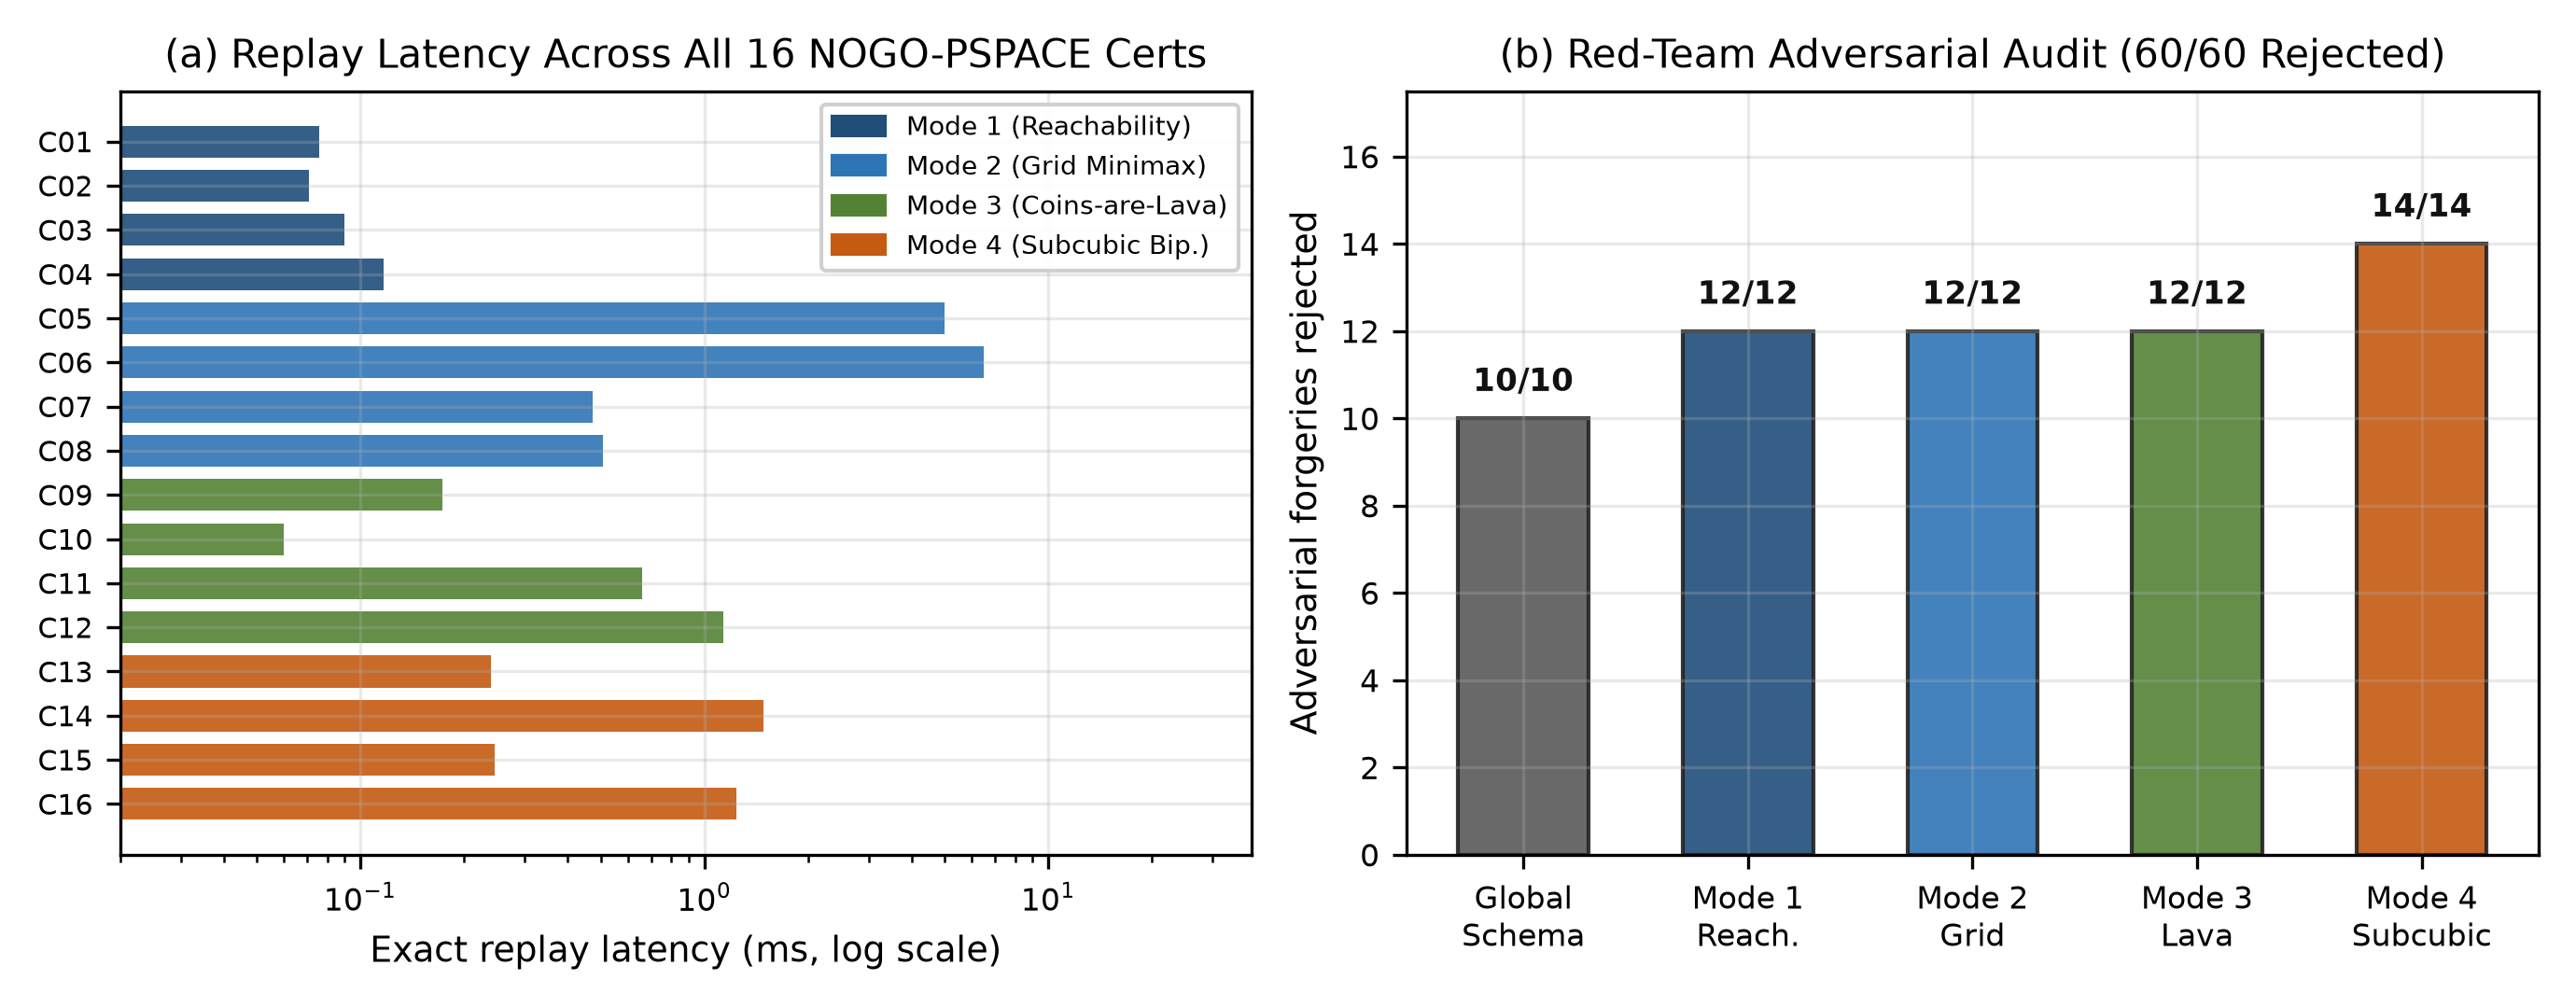
\includegraphics[width=\columnwidth]{../figures/fig3_certificate_replay_atlas.png}
  \caption{(a) Exact zero-float replay latency across all 16 canonical \texttt{NOGO-PSPACE-CERT-1.0} certificates ($0.060$--$6.495\,\mathrm{ms}$). (b) Red-team adversarial audit rejecting 60/60 live forgery attacks.}
  \label{fig:atlas}
\end{figure}

\paragraph{Replay Atlas and Red-Team Audit (Fig.~\ref{fig:atlas}, Table~\ref{tab:replay}).}
All 16 canonical certificates replay in $0.060$--$6.495\,\mathrm{ms}$ with zero floats. Our adversarial suite (\texttt{tests/test\_suite.py}) tests 60 live forgery attacks—including illegal zero-liberty boards, mid-play captures, odd reachability sequences, flipped normal/mis\`ere winners, non-winning claimed first moves, isolated \textsc{Coins-are-Lava} coins, odd-cycle non-bipartite graphs ($C_5$), degree-4 non-subcubic stars ($K_{1,4}$), and disconnected graphs—achieving \textbf{60/60 rejections} with zero bypasses.

\begin{table}[t]
\centering
\caption{Summary of all 16 canonical \texttt{NOGO-PSPACE-CERT-1.0} certificates and 60/60 live adversarial red-team audit.}
\label{tab:replay}
\resizebox{\columnwidth}{!}{%
\begin{tabular}{@{}lccc@{}}
\toprule
Verification Mode & Certs & Latency (ms) & Attacks Rejected \\
\midrule
Mode~1: Grid Legality \& Reachability & 4 & $0.071$--$0.117$ & 12/12 \\
Mode~2: Normal/Mis\`ere Grid Minimax & 4 & $0.472$--$6.495$ & 12/12 \\
Mode~3: \textsc{Coins-are-Lava} Minimax & 4 & $0.060$--$1.138$ & 12/12 \\
Mode~4: Subcubic Bipartite Graph NoGo & 4 & $0.239$--$1.489$ & 14/14 \\
Global Schema / Type / Board & -- & -- & 10/10 \\
\midrule
\textbf{Total} & \textbf{16} & \textbf{0.060--6.495} & \textbf{60/60} \\
\bottomrule
\end{tabular}}
\end{table}

\section{Conclusion}
We delivered an 18-theorem zero-dependency Lean~4 kernel (9 zero-axiom theorems, 0~\texttt{Classical.choice}) and the exact combinatorial game-tree auditor \texttt{NOGO-PSPACE-CERT-1.0} for the finite core of Burke, Davies, and Tennenhouse's PSPACE-completeness proofs for normal/mis\`ere grid \textsc{NoGo} and subcubic bipartite \textsc{Graph NoGo}~\cite{burke2026nogo}. Mechanizing complete planar gadget-embedding coordinates and full B2CL-to-grid compiler verification in Lean~4 remains an exciting next step for formalized combinatorial game theory.

\bibliographystyle{plain}
\bibliography{references}
\end{document}
